%%%%%%%%%%%%%%%%%%%%%%%%%%%%%%%%%%%%%%%%%%%%%%%%%%%%%%%%%%%%%%%%%%%%%%%%%%%%%%%
% Memorial para concurso público de Professor Doutor na USP.
%
% Formatação inspirada em:
% * https://tug.org/pracjourn/2008-1/mori/mori.pdf
% * https://github.com/santisoler/phd-thesis
% * https://github.com/compgeolab/dissertation-template
%%%%%%%%%%%%%%%%%%%%%%%%%%%%%%%%%%%%%%%%%%%%%%%%%%%%%%%%%%%%%%%%%%%%%%%%%%%%%%%

%%%%%%%%%%%%%%%%%%%%%%%%%%%%%%%%%%%%%%%%%%%%%%%%%%%%%%%%%%%%%%%%%%%%%%%%%%%%%%%
% Set a class and import packages
\documentclass[10pt,a4paper,oneside]{book}

% Variables
\newcommand{\Year}{2022}
\newcommand{\Title}{Memorial para concurso público - Professor Doutor em Geofísica - IAG/USP}
\newcommand{\Author}{Leonardo Uieda}
\newcommand{\Email}{Leonardo.Uieda@liverpool.ac.uk}
\newcommand{\ORCID}{0000-0001-6123-9515}
\newcommand{\ResearcherID}{G-3258-2012}
\newcommand{\GoogleScholar}{qfmPrUEAAAAJ}
\newcommand{\Lattes}{8939551682050504}
\newcommand{\GitHub}{leouieda}

\usepackage[utf8]{inputenc}
\usepackage[T1]{fontenc}
\usepackage[brazil]{babel}
\usepackage[width=150mm,top=30mm,bottom=30mm,headsep=10mm,headheight=5mm]{geometry}
\usepackage{graphicx}
\usepackage{amssymb}
\usepackage{amsmath}
\usepackage{hyperref}
% create fancy headers
\usepackage{fancyhdr}
% commands for managing dates and its formats
\usepackage{datetime2}
% improved urls with proper hyphenation
\usepackage{xurl}
% Import enumitem to customize descriptions in license.tex
\usepackage{enumitem}
% Tweak the look of captions
\usepackage{caption}
% To control the style of section titles
\usepackage{titlesec}
% Add the bibliography to the table of contents
\usepackage[nottoc,chapter]{tocbibind}
\usepackage[round,authoryear,sort]{natbib}
% Use custom apalike bibliography style
\bibliographystyle{apalike-doi}
% show dois as links on references
\usepackage{doi}
% Icon fonts (requires using xelatex or luatex)
\usepackage{fontawesome5}
\usepackage{academicons}
\usepackage{fontspec}
% Set fonts (requires compilation with xelatex)
\usepackage{fontspec}
% To make fancy text boxes
\usepackage{xcolor}
\usepackage[framemethod=tikz]{mdframed}
% For fancy and multipage tables
\usepackage{tabularx}
\usepackage{ltablex}
% To define custom environments
\usepackage{environ}
%%%%%%%%%%%%%%%%%%%%%%%%%%%%%%%%%%%%%%%%%%%%%%%%%%%%%%%%%%%%%%%%%%%%%%%%%%%%%%%

%%%%%%%%%%%%%%%%%%%%%%%%%%%%%%%%%%%%%%%%%%%%%%%%%%%%%%%%%%%%%%%%%%%%%%%%%%%%%%%
% Configuration of the document

\setmainfont[%
  Path = fonts/notoserif/,
  UprightFont = NotoSerif-Regular,
  BoldFont = NotoSerif-Bold,
  ItalicFont = NotoSerif-Italic,
  Extension = .ttf
]{NotoSerif}

% Increase the line spacing
\renewcommand{\baselinestretch}{1.5}

% Padding between the first figure and the chapter title
\newcommand{\HeroFigPad}{\vspace{-0.4cm}}

% Add a link to a DOI
\newcommand{\DOILink}[1]{doi:\href{https://doi.org/#1}{#1}}

% Define custom colors
\definecolor{lu_gray}{gray}{0.98}
\definecolor{lu_darkgray}{gray}{0.3}
\definecolor{lu_blue}{RGB}{32, 96, 194}
\definecolor{lu_lightblue}{RGB}{238, 245, 250}
\definecolor{lu_yellow}{RGB}{255, 193, 7}
\definecolor{lu_lightyellow}{RGB}{255, 249, 230}

% Customize how Chapter headings are displayed
\titleformat{\chapter}[display]{\normalfont}{}{5pt}{\vspace{-3.5cm}\huge}[\titlerule]

% Configure captions
\captionsetup{labelfont=bf,font={small,color=lu_darkgray},skip=0pt}

% Define a fancy text box
\mdfdefinestyle{summarybox}{%
  leftline=true,
  rightline=false,
  topline=false,
  bottomline=false,
  linewidth=4pt,
  linecolor=lu_blue,
  frametitlefont=\bfseries\color{black},
  frametitlebackgroundcolor=lu_lightblue,
  frametitleaboveskip=10pt,
  frametitlebelowskip=10pt,
  frametitlerule=true,
  frametitlerulewidth=1pt,
  backgroundcolor=lu_gray,
  innertopmargin=10pt,
  innerbottommargin=15pt,
  innerleftmargin=15pt,
  innerrightmargin=15pt,
}
\newmdenv[style=summarybox]{summarybox}
\mdfdefinestyle{subsummarybox}{%
  leftline=true,
  rightline=false,
  topline=false,
  bottomline=false,
  linewidth=4pt,
  linecolor=lu_yellow,
  frametitlefont=\bfseries\color{black},
  frametitlebackgroundcolor=lu_lightyellow,
  frametitleaboveskip=10pt,
  frametitlebelowskip=10pt,
  frametitlerule=true,
  frametitlerulewidth=1pt,
  backgroundcolor=lu_gray,
  innertopmargin=10pt,
  innerbottommargin=15pt,
  innerleftmargin=15pt,
  innerrightmargin=15pt,
}
\newmdenv[style=subsummarybox]{subsummarybox}

% Define something like an fa-ul and a date list
\NewEnviron{fa-ul}{%
  \vspace{-0.4cm}
  \begin{tabularx}{\linewidth}{@{}p{0.04\linewidth}@{\hspace{0.02\linewidth}}p{0.94\linewidth}@{}}
    \BODY
  \end{tabularx}%
}
\NewEnviron{datelist}{%
  \vspace{-0.4cm}
  \begin{tabularx}{\linewidth}{@{}p{0.15\linewidth}@{\hspace{0.02\linewidth}}p{0.83\linewidth}@{}}
    \BODY
  \end{tabularx}%
}

% Configure hyperref and add PDF metadata
\hypersetup{
    colorlinks,
    allcolors=lu_blue,
    pdftitle={\Title},
    pdfauthor={\Author},
    pdftex,
}

% make urls use the same font as every other text
\urlstyle{same}

% Configure headers and footers
\fancyhf{}
\lhead{\fontsize{10pt}{0}\selectfont\itshape \nouppercase\leftmark}
\chead{}
\rhead{\fontsize{9pt}{0}\selectfont \thepage}
\cfoot{}
\renewcommand{\headrulewidth}{0pt}
%%%%%%%%%%%%%%%%%%%%%%%%%%%%%%%%%%%%%%%%%%%%%%%%%%%%%%%%%%%%%%%%%%%%%%%%%%%%%%%

%%%%%%%%%%%%%%%%%%%%%%%%%%%%%%%%%%%%%%%%%%%%%%%%%%%%%%%%%%%%%%%%%%%%%%%%%%%%%%%
\begin{document}

\pagestyle{plain}
\frontmatter

\begin{titlepage}
  \begin{center}
    
\includegraphics[height=2cm]{images/logo.pdf}
    \vspace{1cm}

    MEMORIAL PARA CONCURSO PÚBLICO

    PROFESSOR DOUTOR (RDIDP) EM MÉTODOS POTENCIAIS

    UNIVERSIDADE DE SÃO PAULO
    \vspace{4cm}

    \textbf{\LARGE \MakeUppercase{\Author{}}}
    \vspace{5cm}

    {\small
      Apresentado para concurso público de títulos e provas para cargo de

      Professor Doutor junto ao Departamento de Geofísica do

      Instituto de Astronomia, Geofísica e Ciências Atmosféricas da

      Universidade de São Paulo.
      \vspace{1cm}

      Edital ATAc-IAG/044/2022
    }
    \vfill

    \Year{}
  \end{center}
\end{titlepage}

%==============================================================================
\chapter*{Resumo}

Resumo curto.
Quem eu sou.
Principais highlights.
Sobre esse memorial (organização etc).
Meu papel no IAG.
Grande parte do texto que está na introdução do memorial antigo.

%==============================================================================
\tableofcontents

\pagestyle{fancy}
\mainmatter

%==============================================================================
\chapter{Introdução}

\begin{figure}[h]
  \HeroFigPad
  \begin{center}
    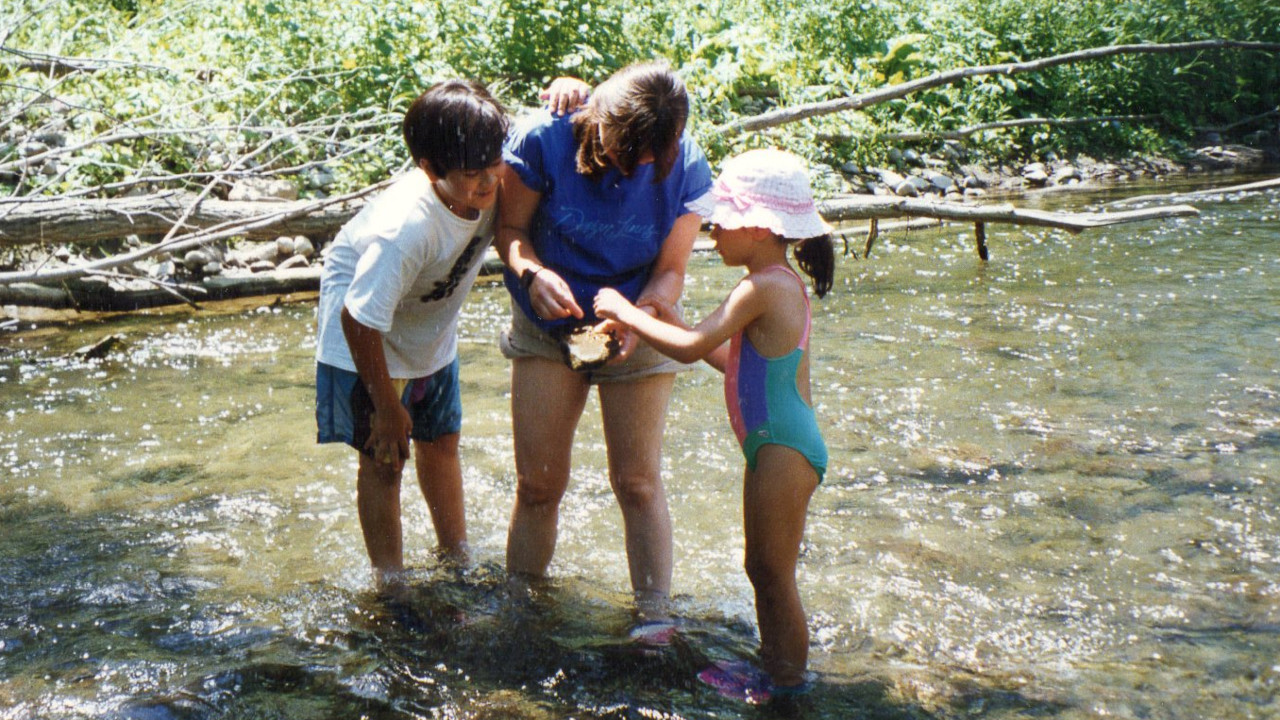
\includegraphics[width=\textwidth]{images/1997-06-ithaca-creek.jpg}
  \end{center}
  \caption{
    Minha mãe mostrando para mim e minha irmã caçula o lado inferior de uma
    pedra em um riacho, provavelmente contendo invertebrados aquáticos.
    Foto de Junho de 1997, tirada no interior do estado de Nova York, E.U.A.,
    durante o pós-doutorado de meus pais na Cornell University.
  }
  \label{fig_riacho}
\end{figure}
\begin{summarybox}[frametitle=\faInfoCircle{}\quad Informações para contato]
  \begin{fa-ul}
    \faEnvelope & email: \href{mailto:\Email}{\Email} \\
    \aiOrcid & ORCID: \href{https://orcid.org/\ORCID}{\ORCID} \\
    \aiLattes & Currículo Lattes: \href{http://lattes.cnpq.br/\Lattes}{lattes.cnpq.br/\Lattes} \\
    \aiPublonsSquare & ResearcherID: \href{https://www.webofscience.com/wos/author/rid/\ResearcherID}{\ResearcherID} \\
    \faUser & Página pessoal: \href{https://www.leouieda.com}{www.leouieda.com} \\
    \faUsers & Grupo de pesquisa: \href{https://www.compgeolab.org}{www.compgeolab.org}
  \end{fa-ul}
\end{summarybox}

\section{Influências}

Sobre meus pais e meu primeiro contato com a pesquisa e ensino superior.
A ética e dedicação eles me passaram.
A oportunidade de morar no exterior.



\section{Privilégio}

Disclaimer sobre meus privilégios.
O memorial é uma reflexão das minhas conquistas.
É importante refletir também nos privilégios que me permitiram chegar onde cheguei.
Nem tudo é mérito.
Suporte familiar.
Classe média e não tive que trabalhar para apoiar meus estudos.
Escola privada.
Oportunidade de morar fora e aprender inglês.
Brasil possui ensino superior gratuito e bolsas.
Ida para o Canada foi financiada pelos meus pais.
Muitas coisas sobre o dia a dia na academia eu já sabia por ver meus pais.
Estigma contra asiáticos é relativamente baixo, pode até ser positivo nas ciências exatas.
Sorte na escolha de curso, ano de ingresso, política a favor da ciência,
professores (Mary Lilian Lourenço, Manoel Roberto Robilotta, Alan Mitchell
Durham) e mentores (Manuel, Ricardo,
Naomi, Val, Carla, Paul), vagas na hora certa, confiança e suporte para reconhecer
opoturnidades e ir atrás.

\section{Estrutura desse memorial}

Como ficou dividido. O que tem em cada parte. Links para os capítulos. Linha do
tempo.

%==============================================================================
\chapter{Formação Acadêmica}

\begin{figure}[h]
  \HeroFigPad
  \begin{center}
    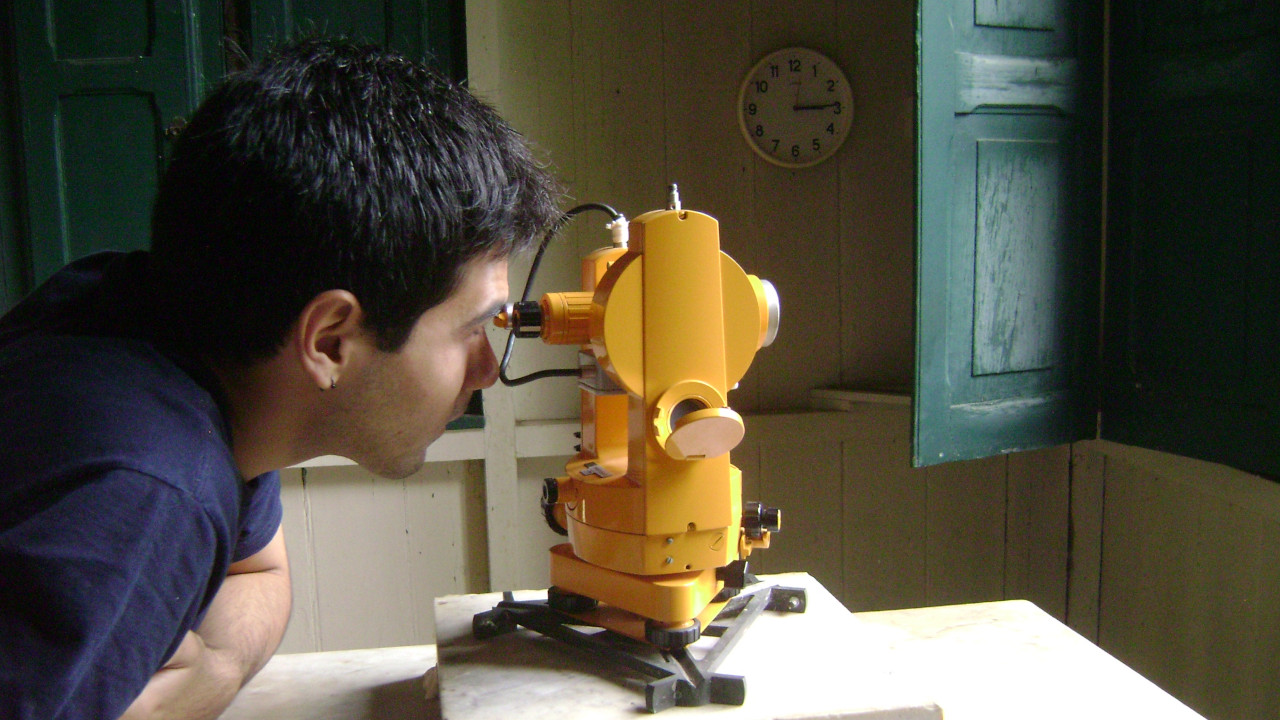
\includegraphics[width=\textwidth]{images/vassouras-geomag-observation-2012.jpg}
  \end{center}
  \caption{
    Realizando medidas da direção do campo geomagnético no observatório de
    Vassouras, RJ. A atividade foi parte de uma disciplina de instrumentação
    geofísica que cursei no mestrado do Observatório Nacional.
  }
\end{figure}
\begin{summarybox}[frametitle=\faGraduationCap{}\quad Bacharelado em Geofísica]
  \begin{fa-ul}
    \faUniversity & Universidade de São Paulo \\
    \faCalendar & Fevereiro 2004 -- Novembro 2009 \\
    \faUser & Orientadora: Naomi Ussami\\
    \aiDoi & \DOILink{10.6084/m9.figshare.963547} \\
    \faInfoCircle & Trabalho de conclusão: Cálculo do tensor gradiente
    gravimétrico utilizando tesseroides
  \end{fa-ul}
\end{summarybox}
\begin{summarybox}[frametitle=\faPlane{}\quad Intercâmbio Internacional]
  \begin{fa-ul}
    \faUniversity & York University, Canadá\\
    \faCalendar & Agosto 2008 -- Maio 2009\\
    \faInfoCircle & Disciplinas de geodésia e posicionamento no curso de
    Engenharia Geomática.
  \end{fa-ul}
\end{summarybox}
\begin{summarybox}[frametitle=\faGraduationCap{}\quad Mestrado em Geofísica]
  \begin{fa-ul}
    \faUniversity & Observatório Nacional \\
    \faCalendar & Fevereiro de 2010 -- Outubro de 2011 \\
    \faUser & Orientadora:  Valéria C. F. Barbosa\\
    \aiDoi & \DOILink{10.6084/m9.figshare.16882300} \\
    \faInfoCircle & Dissertação: Robust 3D gravity gradient inversion by
    planting anomalous densities
  \end{fa-ul}
\end{summarybox}
\begin{summarybox}[frametitle=\faGraduationCap{}\quad Doutorado em Geofísica]
  \begin{fa-ul}
    \faUniversity & Observatório Nacional \\
    \faCalendar & Novembro de 2011 -- Abril de 2016 \\
    \faUser & Orientadora:  Valéria C. F. Barbosa\\
    \aiDoi & \DOILink{10.6084/m9.figshare.16883689} \\
    \faInfoCircle & Tese Modelagem direta e inversão de campos gravitacionais em
    coordenadas esféricas \\
    \faTrophy & Ganhador do Prêmio SBGf de Melhor Tese de Doutorado (2015--2017)\footnotemark
  \end{fa-ul}
\end{summarybox}
\footnotetext{\url{https://sbgf.org.br/premiacoes/}}

Começa de quando ingressei na USP.
Coisas que eu aprendi, IC, TCC, campos, etc.
Turma de graduação e como isso influenciou meu pensamento.
Intercâmbio em York, geodésia, e o
Spiros Pagiatakis\footnote{\url{https://www.yorku.ca/spiros/spiros.html}}.

\section{Universidade de São Paulo}

\section{York University}

\section{Observatório Nacional}

\section{Formação complementar}

\begin{subsummarybox}[frametitle=\faGraduationCap{}\quad The Carpentries Instructor Training]
  \begin{fa-ul}
    \faUniversity & \href{https://carpentries.org/}{The Carpentries} \\
    \faCalendar & 9--10 de Julho de 2018\\
    \faInfoCircle & Habilitação para organizar e ministrar os cursos
    \textit{Software Carpentry}, \textit{Data Carpentry} e
    \textit{Library Carpentry}, incluindo treinamento em pedagogia e práticas
    de ensino de programação e ciência de dados\footnotemark{}
  \end{fa-ul}
\end{subsummarybox}
\footnotetext{\url{https://carpentries.org/instructors/\#leouieda}}
\begin{subsummarybox}[frametitle=\faGraduationCap{}\quad Postgraduate Certificate Academic Practice]
  \begin{fa-ul}
    \faUniversity & Universidade de Liverpool \\
    \faCalendar & Novembro de 2020 -- Maio de 2022 \\
    \faInfoCircle & Curso de pedagogia no ensino superior que me confere o
    título de \textit{Fellow of the Higher Education Academy}\footnotemark{}
    (número de referência PR242069)
  \end{fa-ul}
\end{subsummarybox}
\footnotetext{\url{https://www.advance-he.ac.uk/fellowship/fellowship}}

Esses foram os cursos que deram algum tipo de habilitação especial.

%==============================================================================
\chapter{Atuação Profissional}

\begin{figure}[h]
  \HeroFigPad
  \begin{center}
    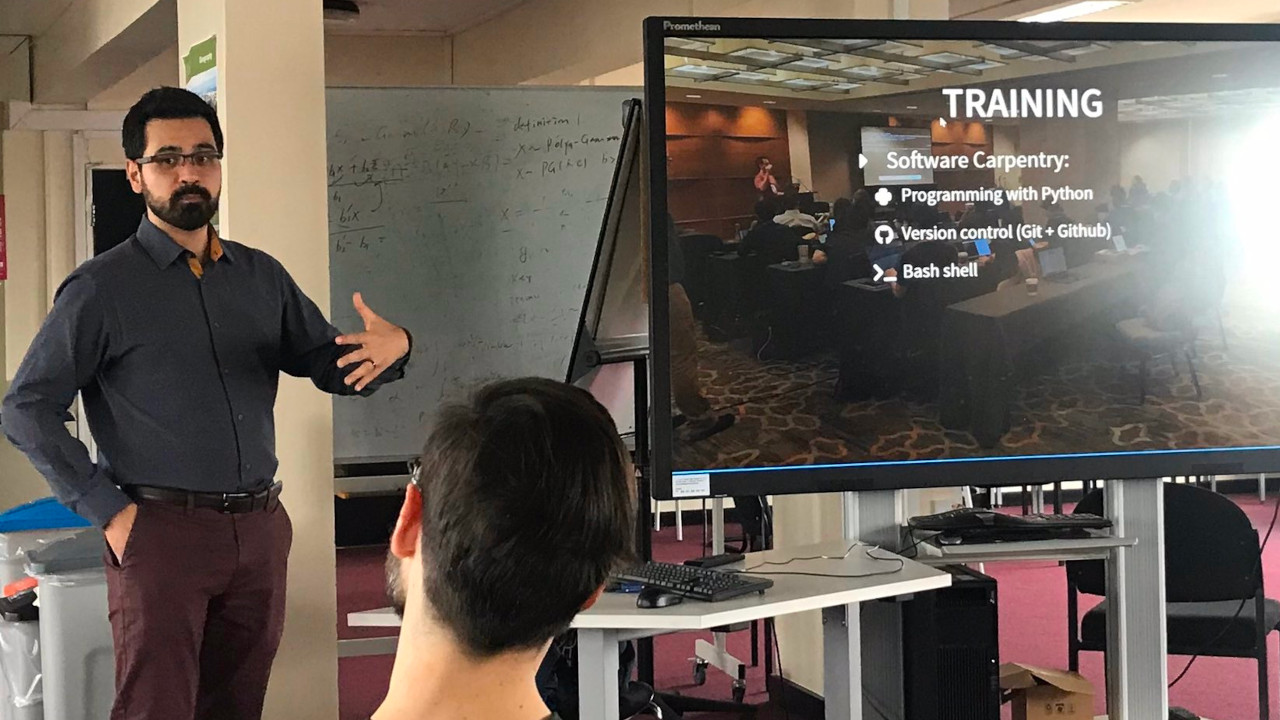
\includegraphics[width=\textwidth]{images/liverpool-gdsl.jpg}
  \end{center}
  \caption{
    Foto de uma apresentação que fiz para o \textit{Geographic Data Science
    Lab} da Universidade de Liverpool em Março de 2020. O propósito da palestra
    era me apresentar para o grupo pouco após minha chegada em Liverpool.
  }
\end{figure}
\begin{summarybox}[frametitle=\faUniversity{}\quad Universidade do Estado do Rio de Janeiro]
  \begin{fa-ul}
    \faUser & Professor Assistente \\
    \faMapMarker & Departamento de Geologia Aplicada -- Faculdade de Geologia \\
    \faCalendar & Fevereiro 2014 -- Janeiro 2018 \\
    \faTrophy & Paraninfo da turma XXX
  \end{fa-ul}
\end{summarybox}
\begin{summarybox}[frametitle=\faUniversity{}\quad University of Hawai`i at M\={a}noa]
  \begin{fa-ul}
    \faUser & Pesquisador Visitante \\
    \faMapMarker & Department of Earth Sciences -- School of Ocean and Earth Science and Technology\\
    \faCalendar & Fevereiro 2017 -- Agosto 2019
  \end{fa-ul}
\end{summarybox}
\begin{summarybox}[frametitle=\faUniversity{}\quad University of Liverpool]
  \begin{fa-ul}
    \faUser & Lecturer (\textit{equivalente a Professor Doutor})\\
    \faMapMarker & Department of Earth, Ocean and Ecological Sciences -- School of Environmental Sciences \\
    \faCalendar & Agosto 2019 -- Presente
  \end{fa-ul}
\end{summarybox}

\section{Universidade do Estado do Rio de Janeiro}

\begin{subsummarybox}[frametitle=\faList{}\quad Atividades Institucionais]
  \begin{datelist}
    2014--2017 & Coordenador: Laboratório de Geofísica de Exploração (LAGEX)\\
    2014--2017 & Coordenador: Projeto Qualitec para contratação de um bolsista de nível superior para atuar no LAGEX\\
    2015--2017 & \textit{Faculty Advisor}: Capítulo Estudantil da Society of
    Exploration Geophysicists (\textit{UERJ Geophysical Society}) \\
    201X & ELEIÇÃO
  \end{datelist}
\end{subsummarybox}

SEG Chapter\footnote{\url{https://seg.org/Education/Student/Student-Chapters/Student-Chapter-Details/student-chapter-listing-details/scID/000000440245}}

Coordenação do LAGEX.

QUALITEC. Victor e Gabriela.

Capítulo SEG.

https://seg.org/Education/Student/Student-Chapters/Student-Chapter-Details/student-chapter-listing-details/scID/000000440245

Eleição

\section{University of Hawai`i at M\={a}noa}

\section{University of Liverpool}

\begin{subsummarybox}[frametitle=\faList{}\quad Atividades Institucionais]
  \begin{datelist}
    2020--2022 & Comissão para avaliação do website do departamento\\
    2020--atual & Early Career Academic (ECA) Representative -- Earth Sciences\\
    2022--atual & Coordenador de curso: Bacharelado em Geofísica e Mestrado em Geologia e Geofísica
  \end{datelist}
\end{subsummarybox}

\section{Atuação na Comunidade Científica}


\begin{subsummarybox}[frametitle=\faList{}\quad Resumo das atividades]
  \begin{datelist}
    2019--2022 & \href{https://joss.theoj.org/}{Journal of Open Source Software}
    (ISSN 2475-9066): Topic Editor \\
    2019--2022 & \href{https://eartharxiv.org/}{EarthArXiv}: Advisory Council Member \\
    2022--atual & \href{https://softwareunderground.org}{Software Underground}:
             Board Member \\
    2022--atual & \href{https://www.pyopensci.org/}{pyOpenSci}:
             Advisory Committee Member
  \end{datelist}
\end{subsummarybox}

JOSS\footnote{\url{https://joss.theoj.org/about\#editors\_emeritus}}

Software Underground\footnote{\url{https://softwareunderground.org/board}}

EarthArXiv\footnote{\url{https://eartharxiv.github.io/AdvisoryCouncil.html}}

pyOpenSci\footnote{\url{https://www.pyopensci.org/our-community/\#pyopensci-working-advisory-committee}}

Revisor de periódicos\footnote{\url{https://www.webofscience.com/wos/author/rid/\ResearcherID}}:
Geophysical Journal International,
Geophysics,
Journal of Geodesy,
Pure and Applied Geophysics,
Journal of Applied Geophysics,
Geophysical Prospecting,
Central European Journal of Geosciences,
Computers and Geosciences
e
Journal of Open Source Software.

Bancas:
2022External PhD thesis examiner (Peter Haas), Christian-Albrechts-Universität zu Kiel.
2022Internal PhD thesis examiner (Yael Annemiek Engbers), University of Liverpool.
2016Internal MSc dissertation examiner (Natacha Medeiros Rocha), Universidade do Estado do Rio
de Janeiro.

Organização de eventos:

%2022 Geo+Code UK.
%2021
%Session: EOS5.3 - The evolving open-science landscape in geosciences: open data, software,
%publications and community initiatives.
%Nijzink, RC, Drost, N, Farquharson, J, Kushnir, A, Pianosi, F, Schymanski, S, Uieda, L, Wadsworth,
%F.
%EGU 2021, Vienna, Austria.
%Session: G4.3 - Acquisition and processing of gravity and magnetic field data and their
%integrative interpretation.
%Ebbing, J, Braitenberg, C, Guy, A, Kaban, MK, Uieda, L.
%EGU 2021, Vienna, Austria.
%2019
%Townhall: Update and Future Directions of the Open-Source Software Initiative.
%Uieda, L, Heagy, LJ, Krischer, L, Gassmoeller, R, Sullivan, CB.
%AGU 2019, San Francisco, USA.
%Session: NS21A - A Tour of Open-Source Software Packages for the Geosciences.
%Heagy, LJ, Gassmoeller, R, Uieda, L, Klump, JF.
%AGU 2019, San Francisco, USA.
%Townhall: The role of an open-source software initiative within the AGU.
%Heagy, LJ, Krischer, L, Uieda, L.
%AGU 2018, Washington DC, USA.


%==============================================================================
\chapter{Ciência Aberta}

\begin{figure}[h]
  \HeroFigPad
  \begin{center}
    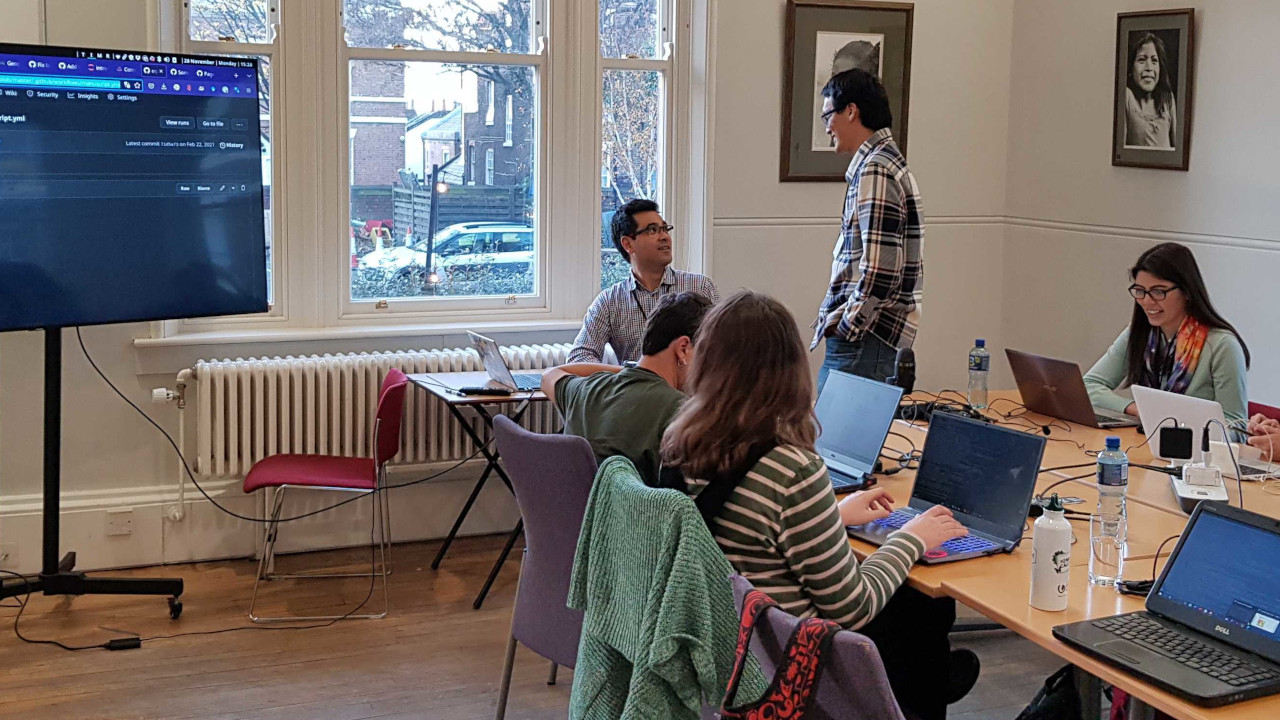
\includegraphics[width=\textwidth]{images/geopluscode.jpg}
  \end{center}
  \caption{
  }
\end{figure}
\begin{summarybox}[frametitle=\faPython{}\quad Software Livre]
  \begin{datelist}
    2008--2016 & Tesseroids (\href{}{}): Criador \\
    2010--atual & Universidade de São Paulo \\
    \faCalendar & Fevereiro 2004 -- Novembro 2009 \\
    \faUser & Orientadora: Naomi Ussami\\
    \aiDoi & \DOILink{10.6084/m9.figshare.963547} \\
    \faInfoCircle & Trabalho de conclusão: Cálculo do tensor gradiente
    gravimétrico utilizando tesseroides
  \end{datelist}
\end{summarybox}
\begin{summarybox}[frametitle=\aiOpenAccess{}\quad Acesso Livre]
  \begin{fa-ul}
    \faUniversity & Universidade de São Paulo \\
    \faCalendar & Fevereiro 2004 -- Novembro 2009 \\
    \faUser & Orientadora: Naomi Ussami\\
    \aiDoi & \DOILink{10.6084/m9.figshare.963547} \\
    \faInfoCircle & Trabalho de conclusão: Cálculo do tensor gradiente
    gravimétrico utilizando tesseroides
  \end{fa-ul}
\end{summarybox}

%==============================================================================
\chapter{Linhas de Pesquisa}

\begin{figure}[h]
  \HeroFigPad
  \begin{center}
    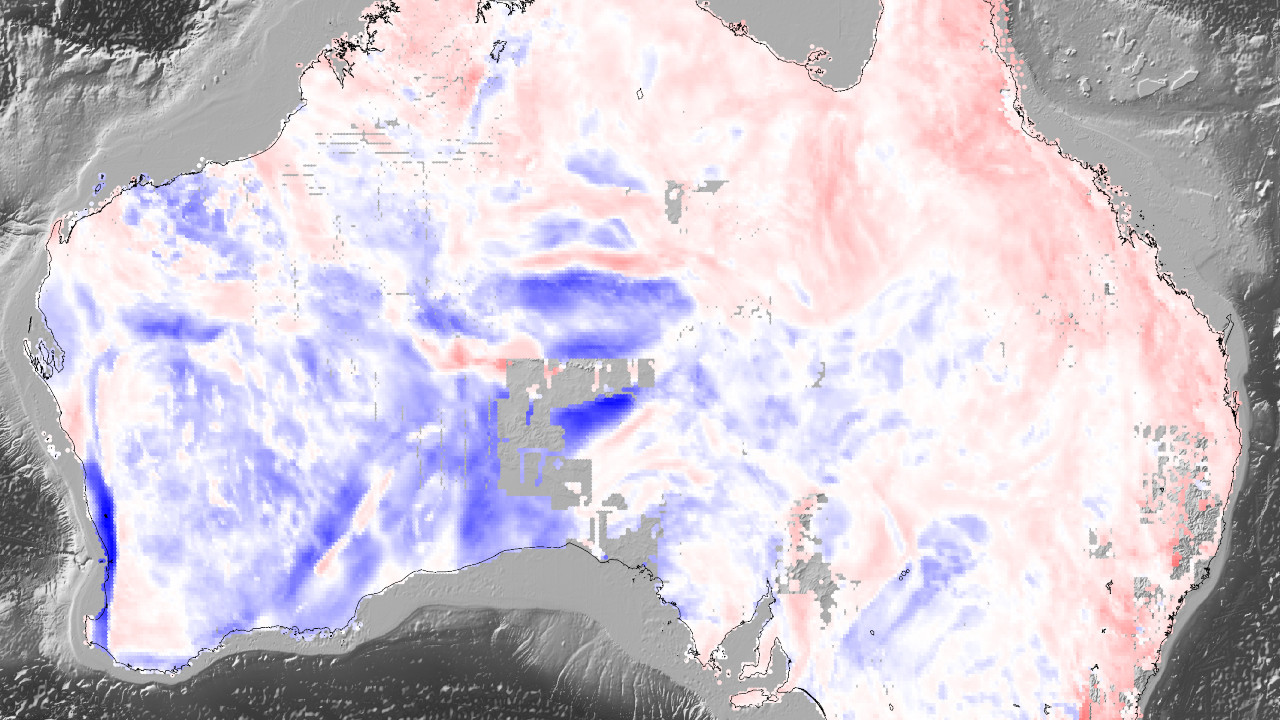
\includegraphics[width=\textwidth]{images/australia-ground-gravity-disturbance.jpg}
  \end{center}
  \caption{
    Bla
  }
\end{figure}
\begin{summarybox}[frametitle=\faLightbulb{}\quad Projetos]
  \begin{fa-ul}
    \faUniversity & Universidade de São Paulo \\
    \faCalendar & Fevereiro 2004 -- Novembro 2009 \\
    \faUser & Orientadora: Naomi Ussami\\
    \aiDoi & \DOILink{10.6084/m9.figshare.963547} \\
    \faInfoCircle & Trabalho de conclusão: Cálculo do tensor gradiente
    gravimétrico utilizando tesseroides
  \end{fa-ul}
\end{summarybox}


%==============================================================================
\chapter{Experiência em Ensino}

\begin{figure}[h]
  \HeroFigPad
  \begin{center}
    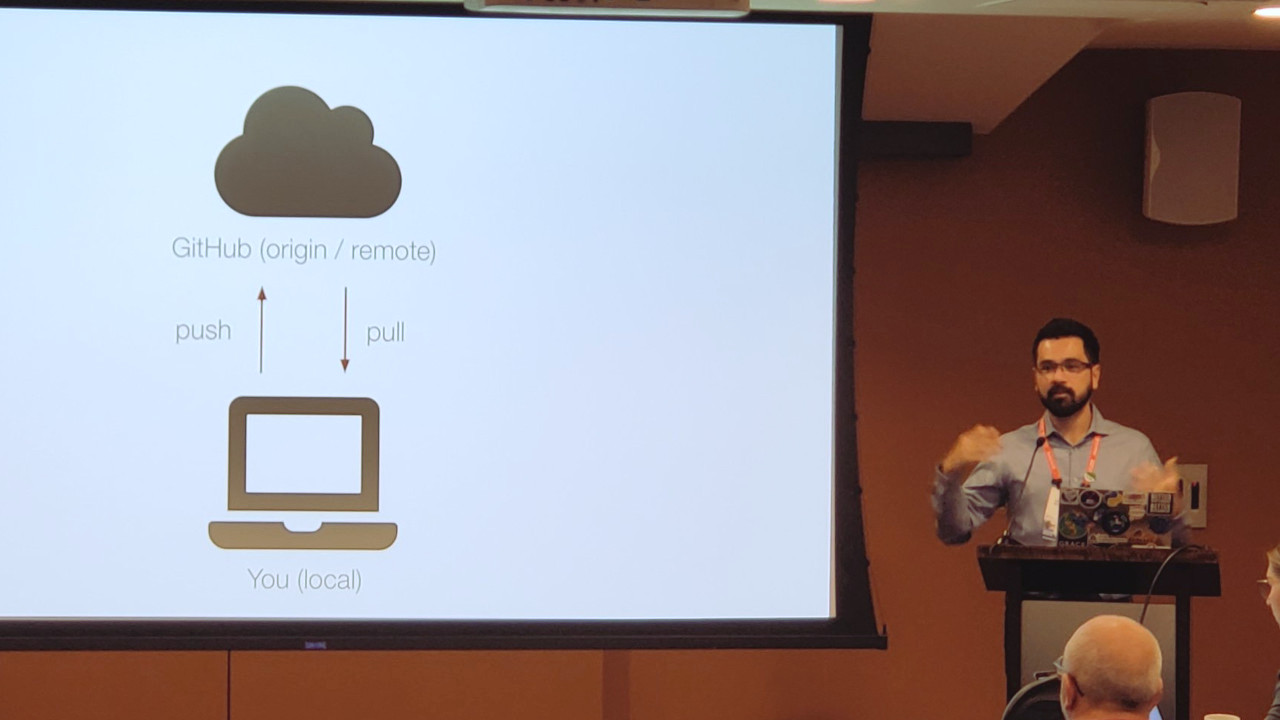
\includegraphics[width=\textwidth]{images/agu-2019-git-lesson.jpg}
  \end{center}
  \caption{
    Bla
  }
\end{figure}
\begin{summarybox}[frametitle=\faChalkboardTeacher{}\quad UERJ]
  \begin{fa-ul}
    \faUniversity & Universidade de São Paulo \\
    \faCalendar & Fevereiro 2004 -- Novembro 2009 \\
    \faUser & Orientadora: Naomi Ussami\\
    \aiDoi & \DOILink{10.6084/m9.figshare.963547} \\
    \faInfoCircle & Trabalho de conclusão: Cálculo do tensor gradiente
    gravimétrico utilizando tesseroides
  \end{fa-ul}
\end{summarybox}

Figura do notebook de ondas sísmicas.


%==============================================================================
\chapter{Conclusão}

Repete resumo dos principais pontos.
Termina com o que eu pretendo conquistar no futuro.

%==============================================================================
\backmatter
%\phantomsection  % use phantomsection to fix bibliography href in the toc
\bibliography{references}

\end{document}
